\documentclass[conference]{IEEEtran}
\IEEEoverridecommandlockouts
% The preceding line is only needed to identify funding in the first footnote. If that is unneeded, please comment it out.
 
\usepackage{amsmath,amssymb,amsfonts}
\usepackage{algorithmic}
\usepackage{graphicx} 
\usepackage{textcomp}
\usepackage{xcolor} 
\usepackage[backend=biber]{biblatex}
\addbibresource{main.bib}

 \def\BibTeX{{\rm B\kern-.05em{\sc i\kern-.025em b}\kern-.08em
     T\kern-.1667em\lower.7ex\hbox{E}\kern-.125emX}}
    
\begin{document}
 
  
\title{Earth at night*\\
{\footnotesize \textsuperscript{*}The visualisation of average radiance in specific area}
}
 
\author{\IEEEauthorblockN{1\textsuperscript{st} Zhen Chen}
\IEEEauthorblockA{\textit{Faculty of Computing and Mathematical Sciences} \\
\textit{The University of Waikato}\\
Beijing, China \\
1561010}
\and
\IEEEauthorblockN{2\textsuperscript{nd} Huajie Xu}
\IEEEauthorblockA{\textit{dept. name of organization (of Aff.)} \\
\textit{name of organization (of Aff.)}\\
City, Country \\
email address or ORCID}
\and
\IEEEauthorblockN{3\textsuperscript{rd} Shengzhu Wang}
\IEEEauthorblockA{\textit{dept. name of organization (of Aff.)} \\
\textit{name of organization (of Aff.)}\\
City, Country \\
email address or ORCID}
\and
\IEEEauthorblockN{4\textsuperscript{th} Wenjie Tong}
\IEEEauthorblockA{\textit{dept. name of organization (of Aff.)} \\
\textit{name of organization (of Aff.)}\\
City, Country \\
email address or ORCID}
\and
\IEEEauthorblockN{5\textsuperscript{th} SiXiang Xiong}
\IEEEauthorblockA{\textit{dept. name of organization (of Aff.)} \\
\textit{name of organization (of Aff.)}\\
City, Country \\
email address or ORCID}
} 

\maketitle

\begin{abstract}
This document is the description about the solution for Assignment 2 of Compx527 paper 
in Waikato University. World Bank Nightime Light Data consists of a lot of satellite imagery 
stored in Amazon Web Services (AWS). Recent files from 2012 to 2020 are generated by the sensor 
named Visible Infrared Imaging Radiometer Suite Day-Night Band (VIIRS DNB) \cite{WorldBan13:online}. All these things are 
stored by Cloud Optimized GeoTIFF (COG) \cite{CloudOpt5:online} format and organized by Spatial Temporal Asset Catalog (STAC) standard \cite{SpatioTe90:online}. 
This project only need the imagery in 3 specific areas, but it is neccessary to process all of them. 
From them, you can learn the trend of their radiance in the period. It is also a good chance to have a better understanding of ecnomic trend by them.
Some researchers also try to find the light pollution by this kind of data \cite{BARA2020106658}.
\end{abstract}

\begin{IEEEkeywords}
Night light, STAC, COG, VIIRS DNB, AWS
\end{IEEEkeywords}

\section{Solution Summary}
A lot of services are depended by this project. It is important to know that imagery from AWS open datasets 
has almost not processed too much before being stored. So the Geospatial Data Abstraction Library (GDAL) is 
imported for the complicated computing. GDAL is a common open source library used for various geospatial data formats \cite{GDAL—GDA74:online}. 
In this project, it is the translator from raster file to vector. So that it is possible to calculate the insection area 
between the satellite imagery and the target area. All of the imagery is the orignal file from the satellite, so
the bad weather would impact the real data, i.e. cloudy and some other atmosphere issues. The project objective is 
to learn the AWS usage and security practice, to get more real data as the reality, more research on how to identify 
cloud and bad weather still need to be done. These bad cases would be influence this project demo very obivously.

In addition, to ensure the development schedule, Lark, which is a kind of instant messenger used in Chinese office, 
is used to record documents and communicate in a group. At the first day, all team members were divided into 7 roles, i.e. project manager,
backend engineer, frontend engineer, devops, testing and data researcher. The project plan was made instantly when everybody understanding
the features, see Fig.~\ref{fig1}.

\begin{figure}[htbp]
    \centerline{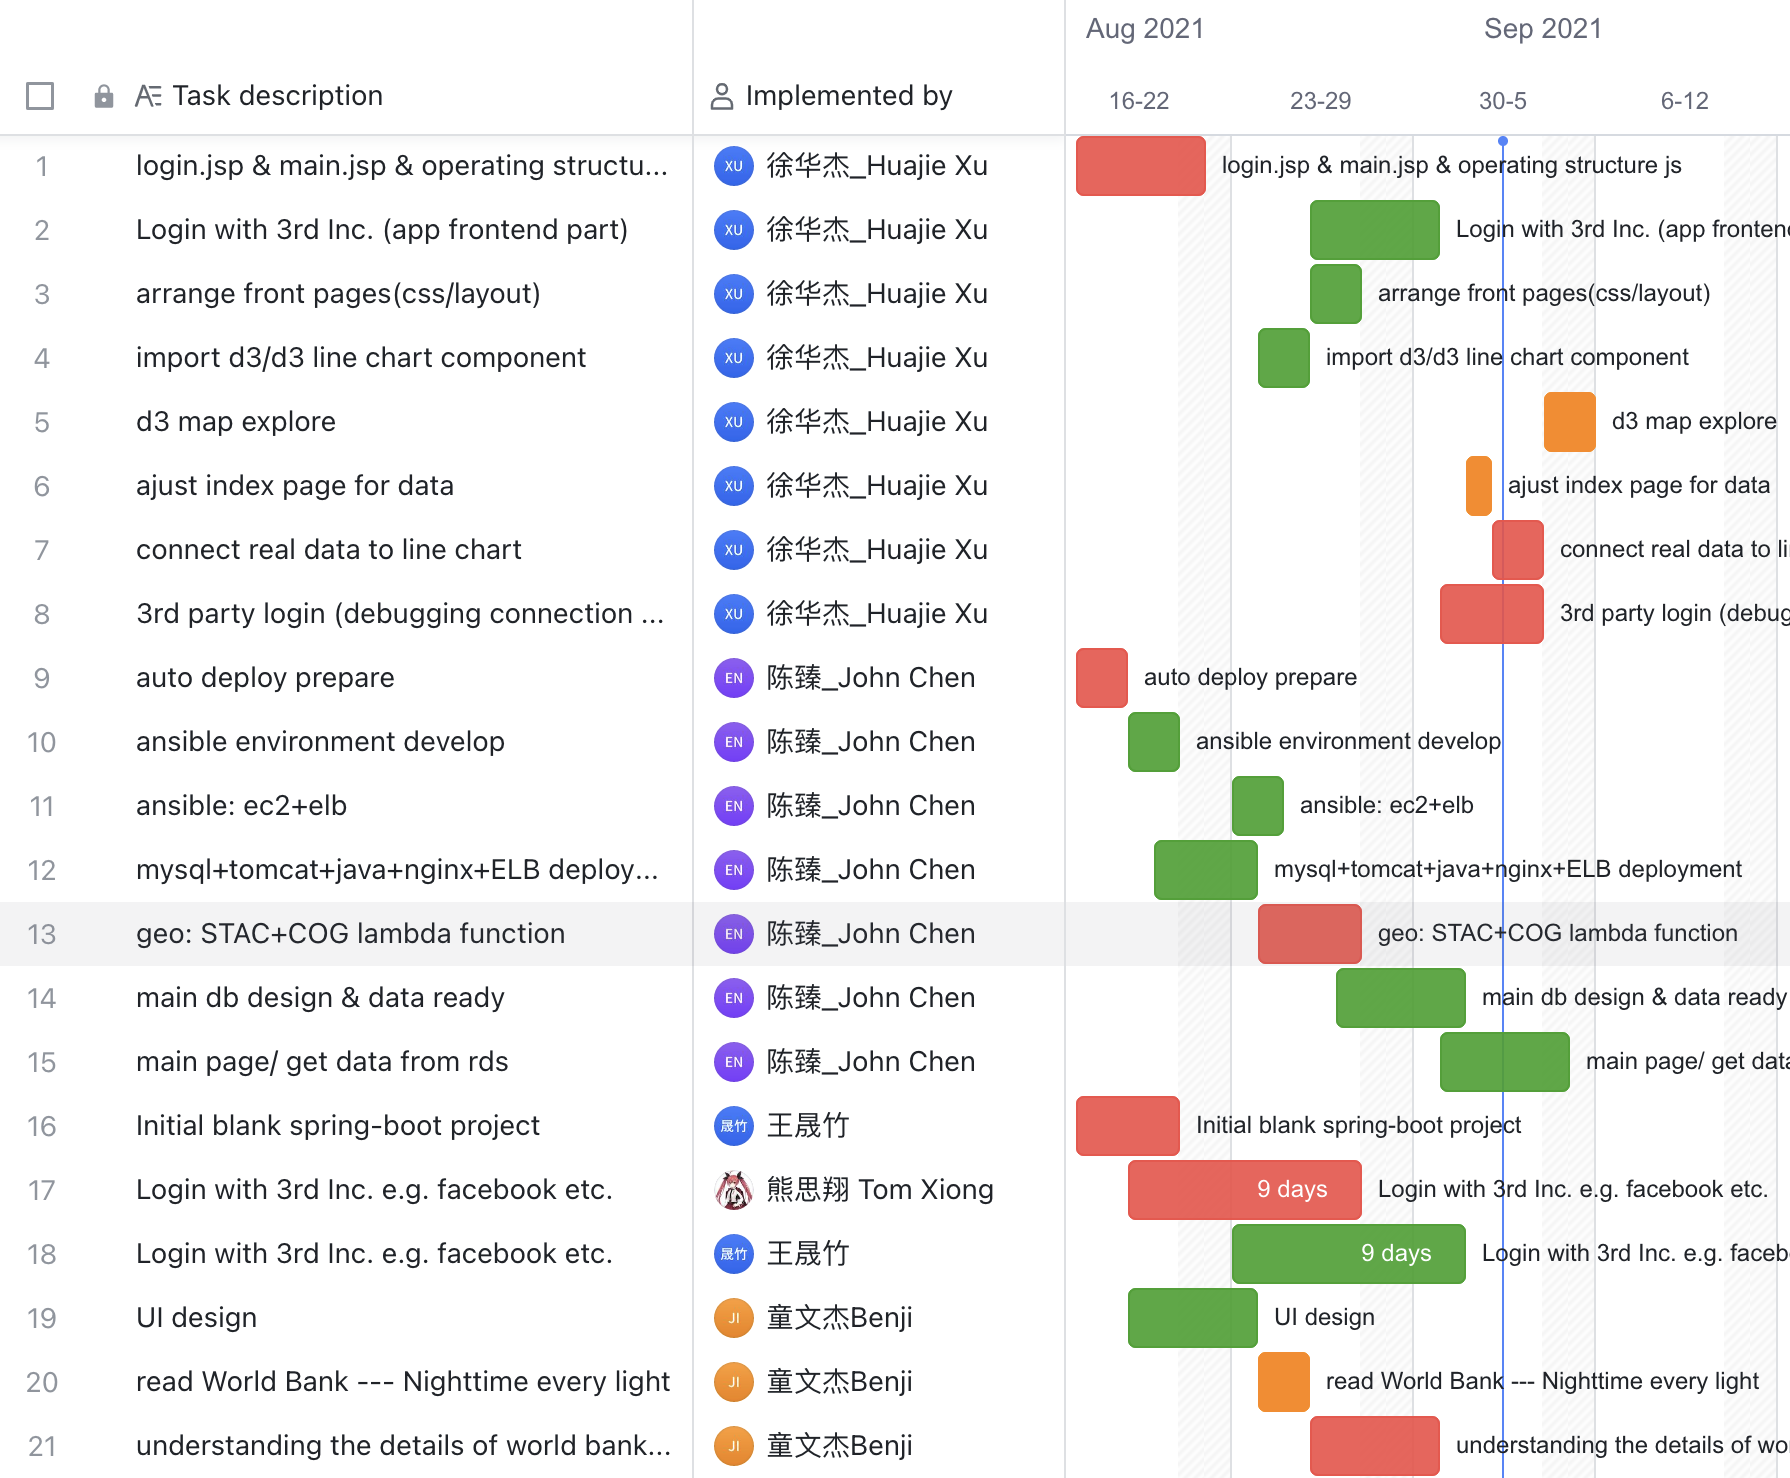
\includegraphics[width=260pt]{images/plan.png}}
    \caption{Project schedule}
    \label{fig1}
\end{figure}

Agile development project management method was used in this project. So the team has a short video meeting everyday. This plan is the last 
result after several development iterations.

The architecture of our solution is shown as Fig.~\ref{fig2}. Both of security and budget are important. So a network address translation (NAT) gateway 
was used for the essential network design. But after two days, NAT had to close because of the budget alert. But it is neccessary that hiding the 
internal services into the internal network instead of exposing them to the internet.

There are two important methods to keep the passowrd safely. The first one is IAM role. IAM role provides good security protection in the whole structure.
Different IAM roles are generated to attach to different Lambda functions. The execution roles are granted permission of access to necessary AWS services. 
There are some common policies for them, e.g. AWSLambdaBasicExecutionRole and AmazonS3FullAccess policies. The second one is Secrets Manager service in AWS.
All of the passwords in this project are stored in it. Visiting it through Secrets Manager when needed.


\begin{figure}[htbp]
    \centerline{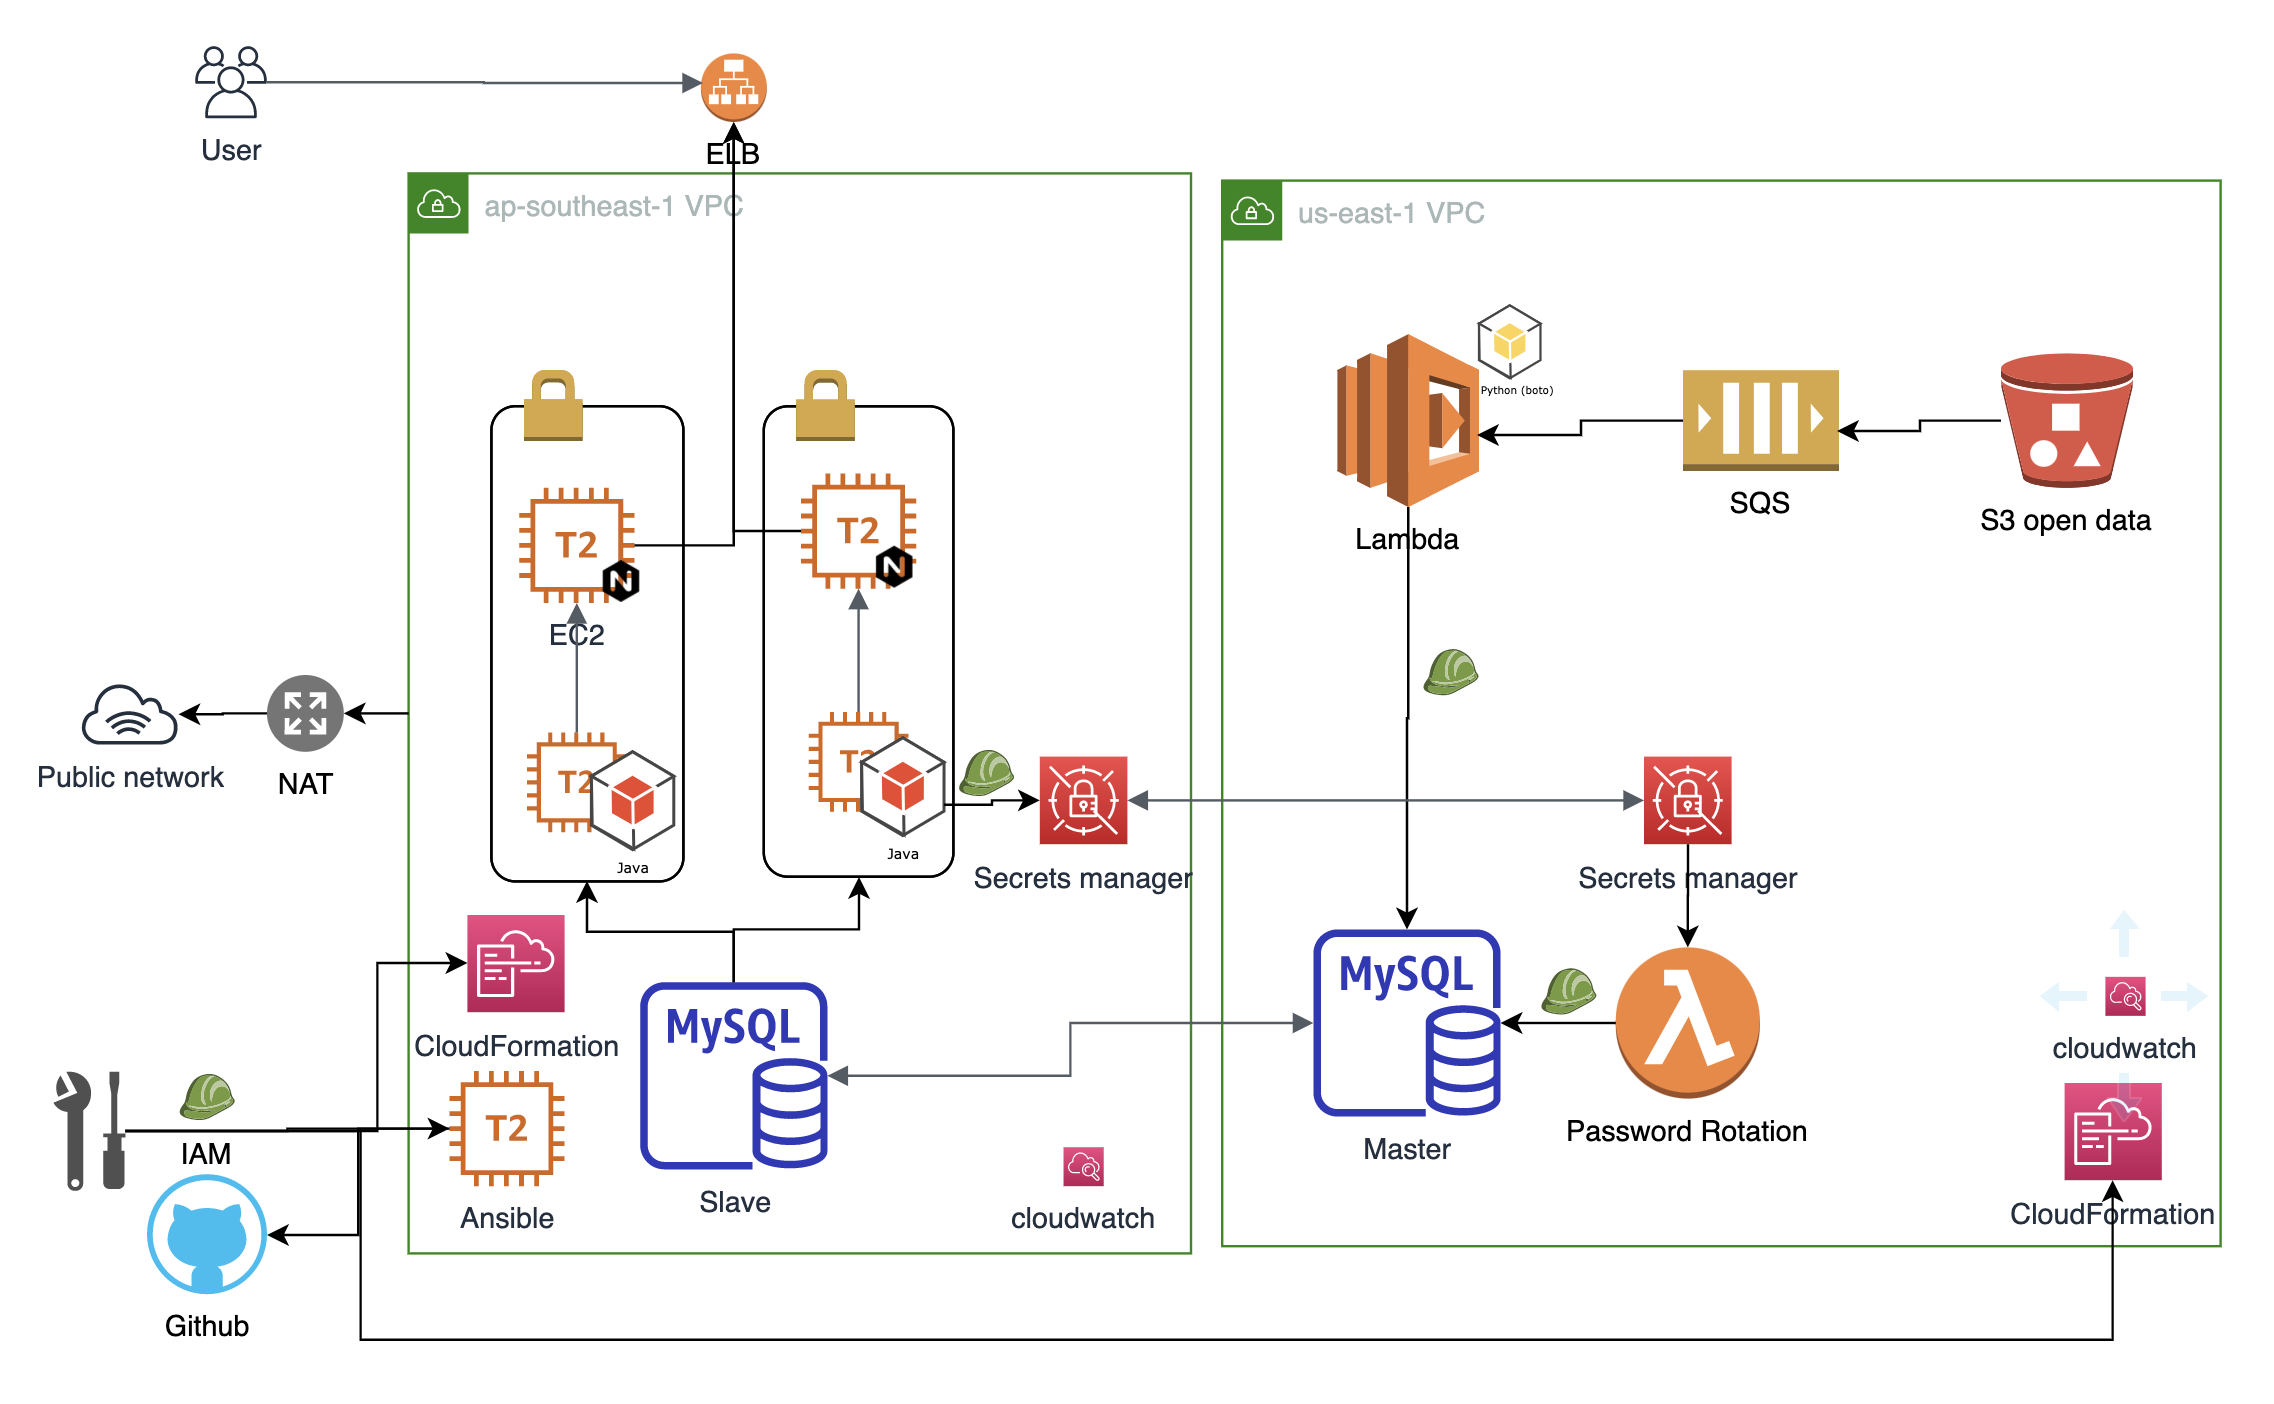
\includegraphics[width=260pt]{images/arch.png}}
    \caption{Architecture}
    \label{fig2}
\end{figure}
    
To process the S3 data, two Lambda functions are generated. One is to follow the STAC protcol to find the imagery, and another is to analyse pictures by GDAL, 
which is a kind of high cost computation in AWS. There are more than 4 pictures per day per area, and about 5,000 pictures per month totally. All the result processed by 
Lambda is stored in RDS and synced from us-east-1 region to ap-southeast-1 region. In addition, the password of MySQL is generated by a Lambda function and rotated 
timely. So the development team do not need to copy the password. Any features with passwords have to get it from Secrets Manager.  

When it comes to show the result in ap-southeast-1 region, network security is the most essential thing because this part of service can be touched by end users. 
So except ELB and the deployment server, there are not any other servers with public IP. All the EC2 instances can visit public network from the NAT, but public network 
can not visit them directly.

To explain more steps, there are some summaries as below. 

\subsection{Open Nighttime Lights}
this is the explaination  \cite{BARA2020106658}

\subsection{Frontend}
this is the explanation

\subsection{Vue}
this is the explanation

\subsection{D3}
this is the explanation
 
\subsection{Spring-boot}
Spring-boot is a Java web framework that can help developer build their web instance very quickly. It is easy to build a 
stand-alone, production-grade application by it \cite{SpringBo66:online}. Because of its features such as no code generation 
and no requirement for XML configuration, it is the best choose for a Java development team.

\subsection{Oauth github}
this is the explanation

\subsection{Ansible}
Ansible is a famous open source deployment platform, which is convenient to enable the infrastructure as code (IaC). 
It is the main tool to deploy most of the services in this project. Especially, a single EC2 instance with public 
IP is provided for it. But AWS service has to provision services by aws-cli instead of Ansible itself. There are still 
some libaries providing these functions but mostly are from external part.

\subsection{CloudFormation}
CloudFormation is a service in AWS, which can organize services very quickly and configure them by yaml or json. There area
several templates for provisioning different services. It is more convient than Ansible for some services. In this project, 
RDS and Lambda Services are dependent on it.

\subsection{Nginx/Tomcat}
Nginx is the widely used web server all over the world. It also has the excellent performance as a reverse proxy. 
Fontend server is the role in this project. Tomcat, which is behind Nginx, is a tranditional Java web container supporting 
Java Servlet. The visualisation is deisgned by Java and run in this container. Both Nginx and Tomcat are well-known because of 
the open source community and internet companies choosing.

\subsection{RDS/Lambda/Secrets Manager/SQS/EC2/NAT}
These items are names of services on AWS. Especially, Lambda are used to generate temperary password of RDS, and store it in 
Secrets Manager. It is really a good method to enhance the security for the password of database. On the other hand, NAT is a 
good feature for isolating the internal and external networks, but the price is too high to be used all the time in this project.

\section{Proposed solution}

A demo has finished all of tasks following the plan on time in this project. But to save budget, stoping NAT and processing parts of data are 
the temporary approaches. It is also possible to deal with the cloud and other disruption to ensure the accrute radiance value. All the 
other details are described as below.

\subsection{Whole infrastructure}
The main architecture is shown as Fig.~\ref{fig2}. First of all, two kinds of IaC platform, which are Ansible and CloudFormation.
Ansible is the first choice that can be esily used in most of situations. When some service need to configure complicatedly, CloudFormation is 
better. Secondly, NAT and ELB are the only entrance to the project. That is the best practice for network security that can mitigate the effects 
of public cyberattacks. Thirdly, IAM roles are used at all kinds of important scenarios, for example, deployment, database visiting, various services visiting.

The source code of entire demo was maintained on Github. The repository URL is https://github.com/A2Inc/A2. There are various languages in it including 
CSS, Vue, Java, JavaScript, Python, Tex. The contributions of team on this demo are shown on Github as Fig.~\ref{fig3}.

\begin{figure}[htbp]
    \centerline{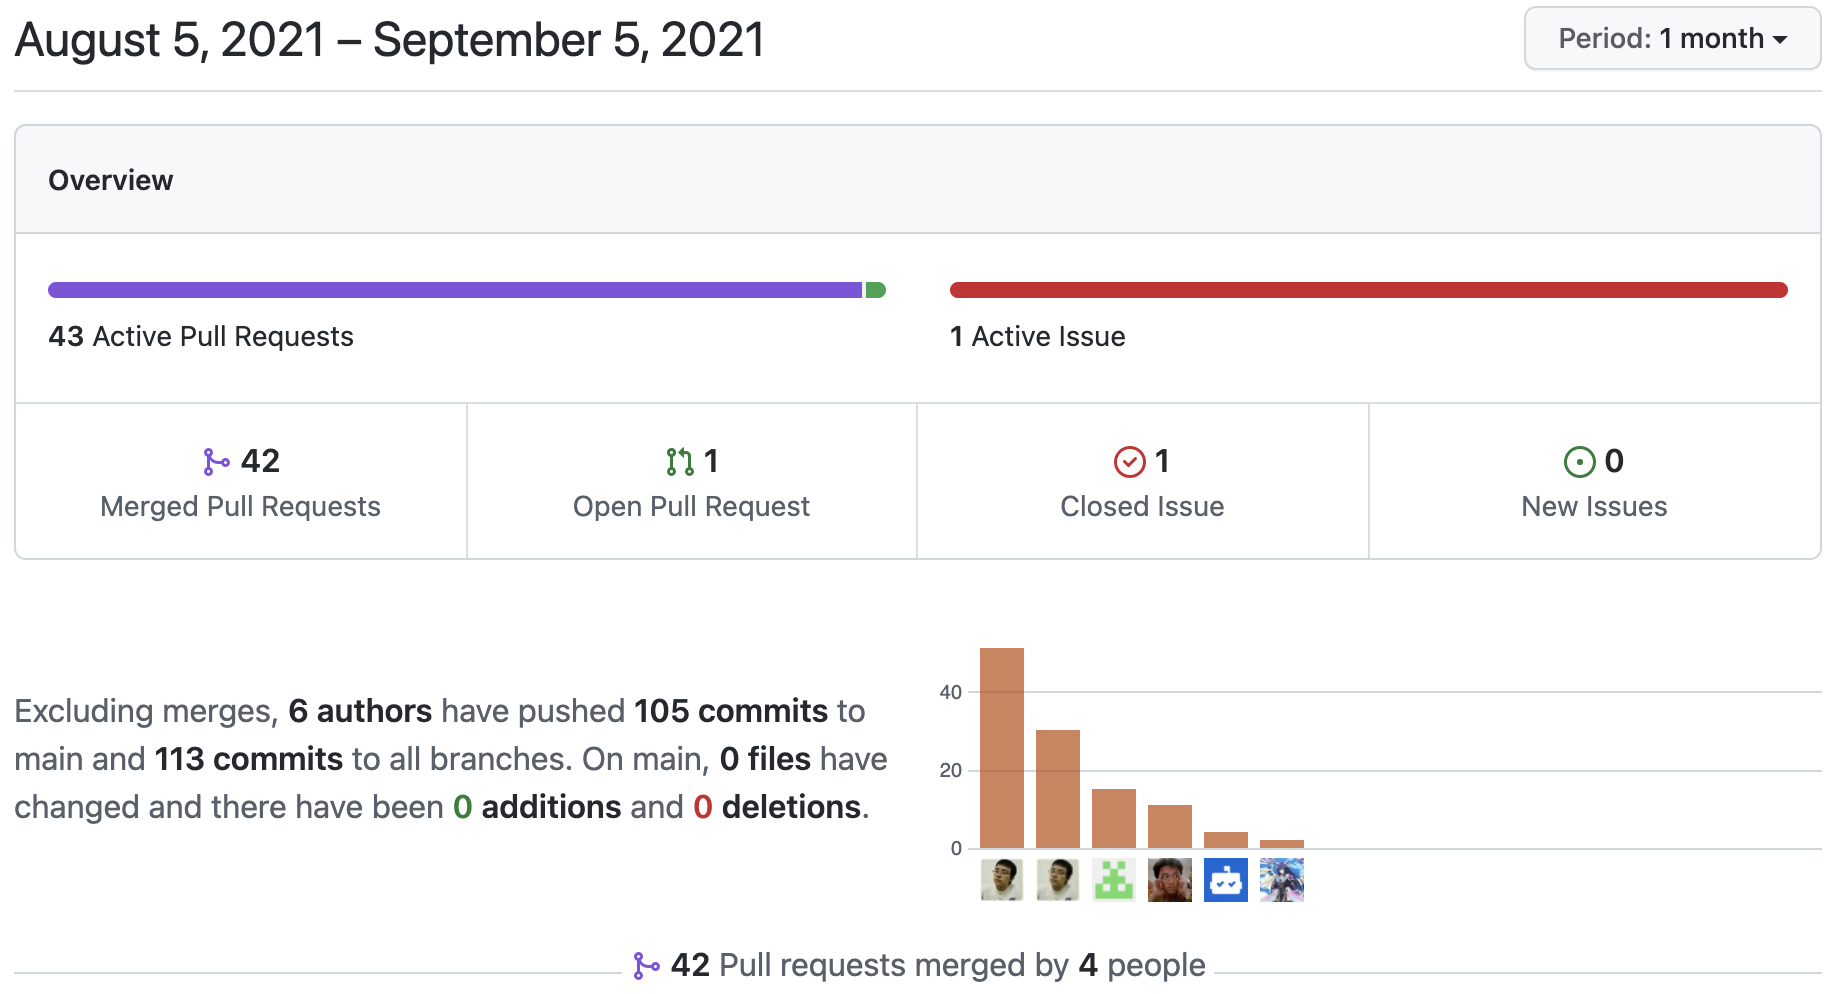
\includegraphics[width=260pt]{images/github.png}}
    \caption{Overview of Github}
    \label{fig3}
\end{figure}

Java, Python and Vue are the most useful tool in this demo. The reason of choosing Java is that almost all of the team members has been good at it. Python 
has a lot of library processing images, so it is the best choice for geospatial imagery. Vue has powerful frontend capabilities, so it is the best for a 
visualisation demo. Latex are used to generate the report and slides.

\subsection{Frontend}

\subsection{Login}
 
\subsection{Data processing}
The pictures in S3 are based on two essential formats, which is STAC and COG. The satellites generate them everyday. World Bank organized the global night lights project 
to store these files in S3. When it comes to deal with the satellite imagery, Python has a lot of easy libraries for geospatial calculating. GDAL is the most useful one. 
It is integrated with Python very well, and is very good at reading and writing raster or vector geospatial file formats.


\begin{figure}[htbp]
    \centerline{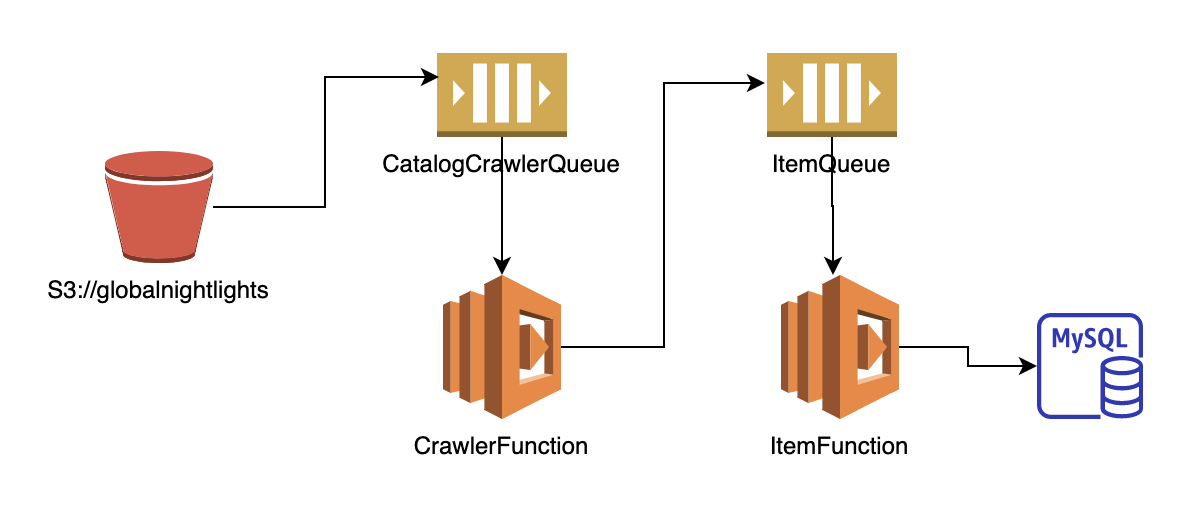
\includegraphics[width=260pt]{images/dataprocess.png}}
    \caption{Data processing}
    \label{fig4}
\end{figure}

Two Lambda functions are used for processing them, shown as Fig.~\ref{fig4}. The first one is to analyse the STAC protocol files. Boundary box can be found from a STAC file, so it is easy to index
all the imagery together by it and then to find the specific area by it. Root STAC file is the first file we processing, which has all of the child links as json files. 
Following the child links, there are the list itmes including the COG file URL. COG file is commonly too large to open directly. GDAL can open it easily and calculate radiance 
value in the file. In the second Lambda function, messages attached COG URL information exchanged by SQS service from the first Lambda function. Because of the complexity 
of GDAL computation, the second Lambda function is slower than the first one.

The second Lambda function is the main logic of the data processing. First of all, choosing cities or areas is a deep issue. The original design was to show the every administrative 
cities. But the global administrative cities geospatial data is very difficult to get. Even though Global Administrative Unit Layers (GAUL) data is provided by Food and 
Agriculture Organization of the United Nation (FAO) \cite{GlobalAd98:online}, the format of these files still needed to research more. So the research areas were reduced 
to three specific areas, such as east of China, Middle East and New Zealand. Secondly, these three areas are defined in advance because they represent the areas of developed, 
developing and war. The radiance of these areas would show very different patterns. And reducing areas can help the function processing more quickly. Thirdly, calculating the 
radiance for every COG file is the core computation. There are intersection areas between the COG file and these three research places. And every pixel in the COG file stores 
a radiance value for this geospatial point. In the World Bank document, there are some special definitions about the value details, such as -999.3 means no-data value, -1.5 
means the beginning of the data range \cite{WorldBan13:online}. The value less than 3 could be disruption value. So all of the numbers which are more than 3 could be the 
sutiable value. At the end, all of the processed information is stored in RDS service. They are date, boundary box, radiance, pixels and so on.

When it comes to the RDS, it is neccessary to introduce the master and slave configuration. Because this global night lights data is stored at us-east-1 region and team members 
use ap-southeast-1 region, master database is installed at us-east-1 region which is closed to S3 data, and slave database is at another region. The cross-region RDS is 
provisioned by CloudFormation because there is a ready template. It has to be mentioned that the cross-region cost is not cheap as other services.


\subsection{Testing}

\subsection{Project management}
Project management is also a big chanllenge in this special period. Scrum development method was chosen from the first day because two of members
had already experienced this method. This iterative approach towards the completion of a project can lead the team to the success.

It is important that some tools let the team work like a native team. All of the team members are from China, but nobody knew each other before. 
So at the first day, the IM platform named Lark, which was widely used in the work place in China, was chosen by team members. Java is the first 
language in the team because team members are almost good at it. By Github, all of the codes can be easily shared with members and easily taken 
control of its version. Remote cooperation is not a easy thing, so team members create a event for vedio meeting everyday. At the same time, it 
is also the agile standup meeting everyday. With the development and research process, some members have to stop to learn more things about the 
lack of relative knowledge. For example, none of members are good at some key technologies, such as geospatial imagery processing, Vue, AWS usage. 
So the development plan was always disrupted because of the learning. Thanks to the agile method, the development is not influenced too much by 
these disruptions. 

Because the members were not sharing the true space in a meeting room, the development atmosphere was a little bit strange. It is difficult to know 
every member's status, so the enthusiasm of development is of critical importance. Somebody went about their tasks with little enthusiasm, and the 
result would be bad at that aspect. At that time, the role of scrum master was very useful, it ensure the entire development schedule.

\section{Security Considerations}
Secruity is the important thing in the development. Although some services can enhance the security, but they are usually very expensive, for example, 
NAT can islote the safer network. There are a lot of details contributing to the security together.

\subsection{IAM}

\subsection{Network}

\subsection{Customer}



\section{Team members and individual contribution within the team}
\begin{itemize}
    \item Zhen Chen:  PM, BE, DevOps
    \item Huajie Xu: FE
    \item Shengzhu Wang(Simon): BE
    \item SiXiang Xiong(Tom): BE, Testing
    \item Wenjie Tong: Data Researcher, Testing
\end{itemize}


\subsection{Figures and Tables}
 Use the abbreviation 
``Fig.~\ref{fig}'', even at the beginning of a sentence.

\begin{table}[htbp]
\caption{Table Type Styles}
\begin{center}
\begin{tabular}{|c|c|c|c|}
\hline
\textbf{Table}&\multicolumn{3}{|c|}{\textbf{Table Column Head}} \\
\cline{2-4} 
\textbf{Head} & \textbf{\textit{Table column subhead}}& \textbf{\textit{Subhead}}& \textbf{\textit{Subhead}} \\
\hline
copy& More table copy$^{\mathrm{a}}$& &  \\
\hline
\multicolumn{4}{l}{$^{\mathrm{a}}$Sample of a Table footnote.}
\end{tabular}
\label{tab1}
\end{center}
\end{table}

\begin{figure}[htbp]
\centerline{
\includegraphics{fig1.png}}
\caption{Example of a figure caption.}
\label{fig}
\end{figure}
 

 
\printbibliography

\end{document}
